\documentclass[12pt]{article}

\usepackage[utf8]{inputenc}
\usepackage{latexsym,amsfonts,amssymb,amsthm,amsmath}
\usepackage{tikz}
\usepackage{stanli}
\usetikzlibrary{calc,through}
\usepackage{multicol}
\usepackage{geometry} 
\usepackage{enumitem}


\setlength{\parindent}{0in}
\setlength{\oddsidemargin}{-0.25in}
\setlength{\textwidth}{7in}
\setlength{\textheight}{9.3in}
\setlength{\topmargin}{-1in}
\setlength{\headheight}{18pt}

\newcommand\blfootnote[1]{%
  \begingroup
  \renewcommand\thefootnote{}\footnote{#1}%
  \addtocounter{footnote}{-1}%
  \endgroup
}

\title{ME473 Dynamic Finite Element Analysis Mini-Project}
\author{Stefano Burzio}
\date{}

\begin{document}
\pagestyle{empty}

\noindent ME473 - Dynamic finite element analysis of structures\hfill EPFL\\
Stefano Burzio \hfill 2025\\
\vspace{0.3cm}

\hspace*{\fill}\textbf{\Large Mini-project 1}\hspace*{\fill}
\begin{center}
  \textbf{\Large Natural frequencies and mode shapes of a uniform shaft}
\end{center}

\hrulefill
\vspace{0.3cm}
\newline
{Project organization:}
\vspace{0.2cm}
\newline
\begin{minipage}[t]{0.38\textwidth}
  \begin{itemize}[itemsep=0.005cm]
    \item Groups: 3 to 4 students
    \item 10\% of final grade
    \item Pdf report: maximum 10 pages
  \end{itemize}
\end{minipage}
\hfill
\begin{minipage}[t]{0.58\textwidth}
  \begin{itemize}[itemsep=0.005cm]
    \item Programming language: \texttt{MATLAB}
    \item Submission: October 31, 2025
    \item Total workload:  32h (approx. 8h per student)
  \end{itemize}
\end{minipage}
\vspace{0.3cm}

\hrulefill
\vspace{0.3cm}

Consider a free-free cylindrical steel shaft of length $\ell = 2\text{ m}$, with a uniform cross-section of radius $r=0.1\text{ m}$, having a polar moment of inertia $I_p$, shear modulus $G=79\text{ GPa}$, and mass density $\rho=7850\text{ kg/m}^{3}$, as shown in the figure below.
\vspace{0.8cm}
\begin{center}
  \begin{tikzpicture}[scale=1]
    % draw lines
    \coordinate (O) at (-6,2);
    \coordinate (P1) at (250:0.5);
    \coordinate (P2) at ($(250:0.5)+(-6,2)$);
    \coordinate (P3) at (70:0.5);
    \coordinate (P4) at ($(70:0.5)+(-6,2)$);
    \draw[fill=gray!40] (P1) -- (P2) -- (P4) -- (P3) -- cycle;
    \draw[thick] (P1) -- (P2);
    \draw[thick] (P3) -- (P4);
    % Draw ellipses
    \draw[thick, fill=gray!40] (0,0) ellipse (0.45cm and 0.5cm);
    \draw[thick,fill=gray!40] (-6,2) ellipse (0.45cm and 0.5cm);

    % draw axis
    \draw[ultra thin,latex-] (1.5,-0.5) node[above] {$x$} -- (-7.5,2.5);
    % length
    \draw[ultra thin] (0,0) -- (0, -2) ;
    \draw[ultra thin] (-6,2) -- (-6, 0) ;
    \draw[latex-latex, ultra thin]  (0,-2)  to node[sloped,midway,above] {$\ell$}(-6,0) ;
    \draw[ultra thin]  (-3,1.2) -- (-1,2) node[right]{$I_p,G,\rho$};
    %origin
    \draw[black,fill=black] (O) circle (.5ex);
    \node[above] at (O) {\small $O$};
    % Draw arc in the middle of the cylinder
    \draw[latex-]
    ($(P1)!0.5!(P2)+(0,-0.5)$)
    arc[start angle=250, end angle=70, radius=1cm]
    node[midway,left] {$\varphi$};
  \end{tikzpicture}
\end{center}
The unknown $\varphi(x,t)$ represents the torsional vibration: the angular displacement (twist angle) at position $x \in[0,\ell]$ and time $t \in[0,T]$.

\begin{enumerate}
  \item[a)] Given the strong formulation for the free vibration problem of the shaft
        $$\begin{cases}
            \frac{\partial}{\partial x}\left(GI_p \frac{\partial}{\partial x}\varphi(x, t)\right) = \rho I_p \ddot{\varphi}(x, t) \\
            GI_p \frac{\partial}{\partial x}\varphi(0, t)=0                                                                       \\
            GI_p \frac{\partial}{\partial x}\varphi(\ell, t)=0                                                                    \\
          \end{cases}$$
        Write the weak formulations, and discretize it using the local approach of the finite element method with $n$ finite elements. Write the expressions for the element mass and stiffness matrices for:
        \begin{itemize}
          \item \textbf{Group A:} linear finite elements,
          \item \textbf{Group B:} quadratic finite elements,
          \item \textbf{Group C:} cubic finite elements.
        \end{itemize}
  \item[b)] Determine the first $5$ approximate natural frequencies and mode shapes of the shaft for $n = 1,\, 2,\, 4,\, 8$, and $16$ finite elements. Compare the results with the exact natural frequencies obtained from the analytical solution, and analyze the convergence of the numerical predictions.
  \item[c)] Discuss qualitatively the influence of the boundary conditions (free-free, clamped-free, clamped-clamped) on the approximated natural frequencies and mode shapes.
\end{enumerate}

\end{document}